\documentclass{standalone}
\usepackage[dvipsnames, fixpdftex]{xcolor}
\usepackage{tikz}

\begin{document}
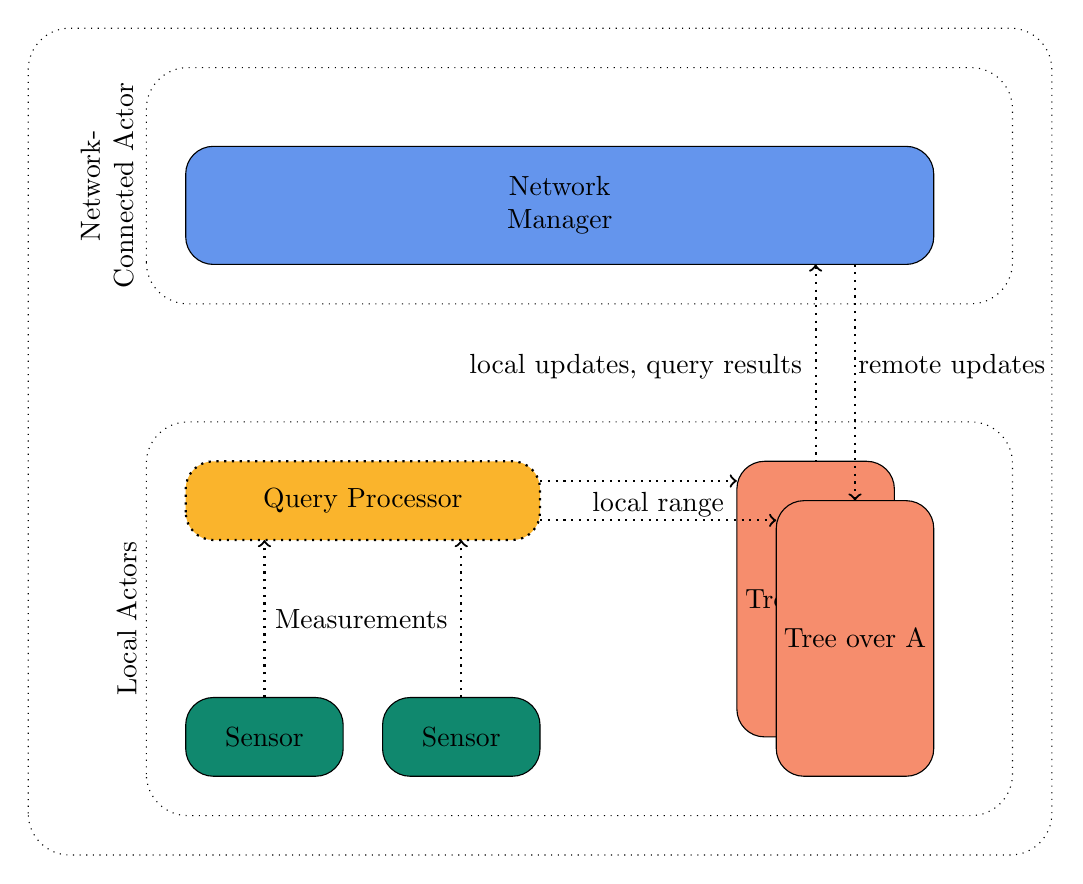
\begin{tikzpicture}
    % Reference coordinates
    \coordinate (tA) at (8.5,4.25);
    \coordinate (tAtop) at (9.5,4.5);
    \coordinate (tB) at (8,4.75);
    \coordinate (tBtop) at (9,5);
    \coordinate (nmtA) at (9.5,7.5);
    \coordinate (nmtB) at (9,7.5);
    \coordinate (sens1) at (2,2);
    \coordinate (sens2) at (4.5,2);
    \coordinate (qp1) at (2,4);
    \coordinate (qp2) at (4.5,4);
    \coordinate (qptop) at (3.25,5);
    \coordinate (qprightB) at (5.5, 4.75);
    \coordinate (qprightA) at (5.5, 4.25);
    \coordinate (nmqp) at (3.25,7.5);
    % Frames
    \draw[rounded corners=15pt, dotted] (-1,0) rectangle (12,10.5);
    \draw[rounded corners=15pt, dotted] (0.5,0.5) rectangle (11.5,5.5) node[rotate=90, pos=0.5, yshift=5.75cm]{Local Actors};
    \draw[rounded corners=15pt, dotted] (0.5,7) rectangle (11.5,10) node[rotate=90, pos=0.5, yshift=6cm, align=center]{Network-\\Connected Actor};
    % Trees
    \draw[rounded corners=10pt, fill=Melon] (8,1.5) rectangle (10,5) node[pos=0.5]{Tree over B};
    \draw[rounded corners=10pt, fill=Melon] (8.5,1) rectangle (10.5,4.5) node[pos=0.5]{Tree over A};
    % Network Manager
    \draw[rounded corners=10pt, fill=CornflowerBlue] (1,7.5) rectangle (10.5,9) node[pos=0.5, align=center]{Network \\ Manager};
    % Query processing
    \draw[rounded corners=10pt, dotted, thick, fill=Dandelion] (1,4) rectangle (5.5,5) node[pos=0.5, yshift=0em]{Query Processor};
    % Sensors
    \draw[rounded corners=10pt, fill=PineGreen] (1,1) rectangle (3,2) node[pos=0.5, yshift=0em]{Sensor};
    \draw[rounded corners=10pt, fill=PineGreen] (3.5,1) rectangle (5.5,2) node[pos=0.5, yshift=0em]{Sensor};
    %  sensor - qp Lines
    \draw[->, dotted, thick](sens1) to node[pos=0.5, xshift=3.5em]{Measurements} (qp1);
    \draw[->, dotted, thick](sens2) to (qp2);
    % qp - tree lines
    \draw[->, dotted, thick] (qprightA) to node[pos=0.5, yshift=2mm]{local range} (tA);
    \draw[->, dotted, thick] (qprightB) to (tB);
    % Nm lines    
    \draw[->, dotted, thick] (nmtA) to node[pos=0.5, xshift=3.5em,yshift=2mm]{remote updates} (tAtop);
    \draw[<-, dotted, thick] (nmtB) to node[pos=0.5, xshift=-6.5em,yshift=-0.5mm]{local updates, query results} (tBtop);
\end{tikzpicture}
\end{document}